\documentclass[11pt,letterpaper]{article}
\usepackage{graphics}
\usepackage{fullpage}
\addtolength{\voffset}{0.5in}

%
%  Cool LaTeX resource:
%   http://en.wikibooks.org/wiki/LaTeX

\begin{document}

\bibliographystyle{plain}

\title{Bayesian Knowledge Tracing and the Identifiability Problem}
\author{Brett van de Sande}

\maketitle

\begin{abstract}
The Bayesian Knowledge tracing model is very widely used in
modeling student learning.  Unlike most Hidden Markov Models,
it is simple enough that it can be solved analytically, which
gives some insight into its behavior.  In particular, we show that
it is, in fact, a model with three parameters and has the 
functional form of an exponential.
\end{abstract}

%
%  Had idea to look at extensions to BKT where the analytic solution
%  is  not feasible but use variation of parameters to find any
%  "identifiability problem" (degeneracies).  However, the two that I
%  know about, Lee and  Brunskill and Baker's models do not have any 
%  degeneracies.   Probably not worth the effort, since a random, very 
%  complicated model, in general, will not have any degeneracies.
%


\section{Introduction}

The Bayesian Knowledge Tracing (BKT) model was first introduced by Corbett
and Anderson~\cite{corbett_knowledge_1994}.  Since then, it has been widely applied
in studies of student learning.  In addition, it often serves as the starting
%
%   Need examples of BKT-based models, only look at examples
%   where identifiability problem exists.
%
point for more complicated models of learning, for example~\cite{baker_r._improving_2008,lee_impact_2012}.  
While using this model,  number of authors have noted have noted the 
existence of what is called the ``identifiability problem'' \cite{beck_identifiability:_2007}.    
That is, there are certain combinations of the model 
parameters that produce identical models.   

The BKT model is commonly expressed as a Hidden Markov Model (HMM).
A typical HMM must be solved numerically to find its functional form.
However, the BKT model is simple enough that it can be solved analytically,
which we will do here.  We will see that the model, in functional
form, is an exponential.  Moreover, we will see that it is, in fact,
a three parameter model, explaining the identifiability problem.

%There are several reasons why a HMM is a good represention.  First,
%the parameters of the HMM are often thought to have some physical
%significance.  In BKT, for instance, $P_j$ is the probability that the
%student knows the skill at a certain point of time:  it is a simple
%mental model of the student.  Thus, a distinction can be made between
%the student's mental state and their actual behavior (whether they
%can apply the skill correctly).   In contrast, a more behaviorist
%approach would eschew $P_j$ in favor of a model of actual behavior.


\section{Bayesian Knowledge Tracing}

The Bayesian Knowledge Tracing model~\cite{corbett_knowledge_1994} has four parameters:
%
\begin{itemize}
   \item $P_0$ is the initial probability of knowing a skill.
   \item $P(G)$ is probability of guessing correctly, if the student        
         doesn't know the skill.
   \item $P(S)$ is probability of slips, if student does know the skill.
   \item $P(L)$ is probability of learning the skill if the student 
         does not know the skill.  Note that $P(L)$ is assumed to 
         be constant over steps.
\end{itemize}
%
Let $P_j$ be the probability that the student knows the skill at 
step $j$. According to the model,  $P_j$ can
be determined in terms of the previous opportunity:
%
\begin{equation}
          P_j = P_{j-1} + P(L)\left(1-P_{j-1}\right)  \; . \label{recurse}
\end{equation}
%
According to this model, the probability that the student actually gets
opportunity $j$ correct is:
%
\begin{equation}
         P_j(C) = P(G)\left(1-P_j\right) + \left(1-P(S)\right) P_j \; . \label{pnc}
\end{equation}
%
(Unlike the four model parameters above, there isn't a consistent
notation for $P_j(C)$ in the literature.)

This model can be  solved exactly.  First, we rewrite (\ref{recurse}) in a
more suggestive form:
%
\begin{equation}
        1-P_j = \left(1-P(L)\right) \left(1-P_{j-1}\right) \; .
\end{equation}
%
One can show that this recursion relation has solutions of the form:
%
\begin{equation}
            1-P_j = \left(1-P(L)\right)^j\left(1-P_0\right) \; .
	    \label{sol}
\end{equation}
%
%
Substituting (\ref{sol}) into (\ref{pnc}), we get:
%
\begin{equation}
         P_j(C) = 1-P(S) -\left(1-P(S)-P(G)\right) \left(1-P_0\right)
                   \left(1-P(L)\right)^j \; . \label{pncsoln}
\end{equation}
%
Note that the functional form of $P_j(C)$ is a function of {\em three}
parameters:  $P(S)$, $P(L)$, and $\left(1-P(S)-P(G)\right) \left(1-P_0\right)$.

The functional form of (\ref{pncsoln}) is an exponential.
If we define
%
\begin{equation} 
          A=\left(1-P(S)-P(G)\right) \left(1-P_0\right)  \label{aa}
\end{equation}
%
 and $\beta=-\log(1-P(L))$, then we can rewrite (\ref{pncsoln}) in 
a clearer form:
%
\begin{equation}
         P_j(C) = 1-P(S) -A e^{-\beta j} \, ;
\end{equation}
%
see Fig.~\ref{bktgraph}.

\begin{figure}
\centering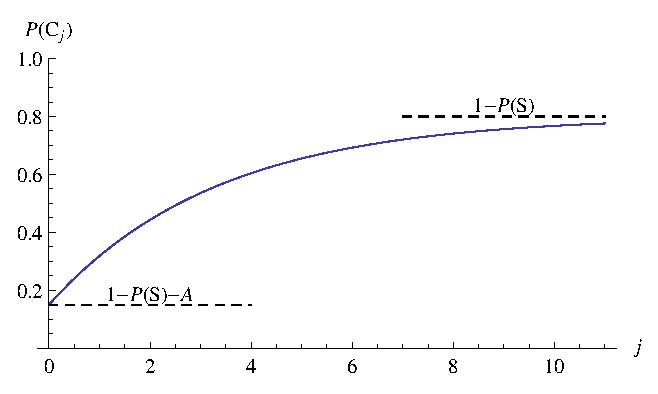
\includegraphics{exponential.eps}
\caption{The Bayesian Knowledge Tracing model in functional form. 
          $P_j(C)$ the probability of  the student getting step $j$ correct.}
 \label{bktgraph}
\end{figure}

\section{Identifiability and Model Degeneracy}

The fact that the BKT model is a function of three parameters
was first noticed by Beck and Chang~\cite{beck_identifiability:_2007} 
where they call it the ``identifiability problem.''   In their paper, they noteed that multiple
combinations of $P(G)$ and $P_0$ give exactly the same $P_j(C)$, but
failed to explain why this is the case.  An example showing the relation
between $P(G)$ and $P_0$ for a given model is shown in Fig.~\ref{table1}.

Baker and co dicsuss the need for paramters to.
Let us use parameters from Table~1 of
\cite{beck_identifiability:_2007} for the BKT model: 
$P(S)=0.05$, $P(T)=0.1$, and $A=0.418$.

\begin{figure}
\centering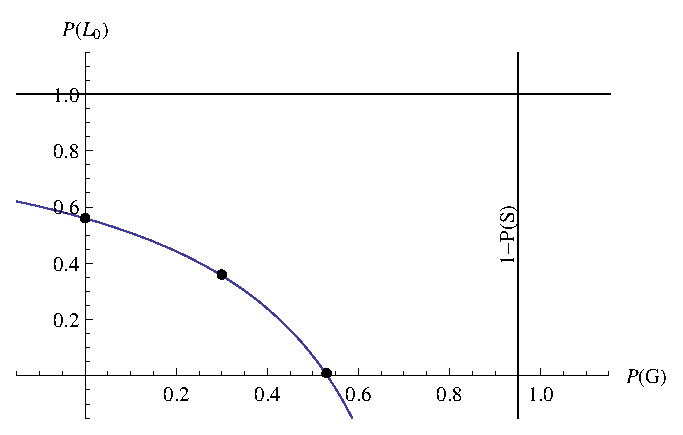
\includegraphics{table1.eps}
\caption{Relation between $P(G)$ and $P_0$ for the BKT model in Table~1
  of \cite{beck_identifiability:_2007}.  The three points are the
  three models in Table~1 of \cite{beck_identifiability:_2007}.  The
  line is from Eqn.~\ref{aa}, with $P(S)=0.05$ and $A=0.418$. }
 \label{table1}
\end{figure}


\section{Conclusion}

In conclusion, the Bayesian Knowledge Tracing model, when expressed
in functional form, is an exponential function with three parameters.
It is unclear how the identifiability problem has affected previous
results.  Certainly, any study that relies on a value for $P(G)$ or
$P_0$ as output from a fit to student data would be affected.
On the other hand, studies that rely only on $P(S)$ or $P(L)$ from
a fit to student data should be OK.  In addition, expressing
the model in terms of three parameters should improve speed
and accuracy of any maximum likelihood fit to student data.

Some authors have addressed the identifiability problem by 
% paper with work-around for identifiability problem (Aleven?)
%
% Dynamic Cognitive Tracing: Towards Unified Discovery of 
% Student and Cognitive Models  Jose P. Gonzalez-Brenes and Jack
% Mostow  set P_0=0.
fixing $P_0$ using some additional constraint~\cite{fix}.  
This is of use in the case where, after fitting the model to data, 
$P(G)$ a being used as a model output.  Otherwise, the impsition
of the additional constraint has no effect on the result.

% Question:  can Markov chains produce power law behavior? YES!
% Need supporting literature for power law vs. exponential.

Finally, we see that the functional form of BKT corresponds 
to an exponential, rather than a power law.  
Heathcote, Brown, and Mewhort~\cite{heathcote_power_2000}
argue that learning for individuals is better described by
exponentials while (as shown in earlier studies) learning averaged
over individuals is better described by a power law function.
This suggests that BKT may be more appropriate for describing
individual learners, rather than performance averaged over students.


%Equations (1) and (2) of \cite{lee_impact_2012} 
%are equivalent to the first three equations in \cite{baker}
%\begin{eqnarray}
%   P(L_n|\mbox{correct}) &=& P(T)+\frac{\left(1-P(T)\right) P(L_{n-1})
%          \left(1-P(S)\right)}
%               {P(L_{n-1})\left(1-P(S)\right)+\left(1- P(L_{n-1})\right) P(G)}\\
%   P(L_n|\mbox{incorrect}) &=& P(T)+\frac{\left(1-P(T)\right) P(L_{n-1})
%          \P(S)\right}
%               {P(L_{n-1})P(S)+\left(1- P(L_{n-1})\right) \left(1-P(G)\right)}\\
%with the substitution:
%
%\begin{equation}
%         P(L_{n-1}) \to P(T)+\left(1-P(t)\right) p(L_t)
%\end{equation}
%
%This equivalence is from changing the order of updating
%student mastery and updating the estimate based on student
%response, as noted by the authors.  However, this raises
%a question for Equations (3) and (4) of \cite{lee_impact_2012}.
%Should the probability be taken before or after updating the
%student mastery:

\bibliography{education-modeling}

\end{document}